\documentclass[article]{jss}
\usepackage{amsmath,thumbpdf,lmodern}
\graphicspath{{Figures/}}

\newcommand{\x}{\mathbf{x}}
\newcommand{\tild}{\symbol{126}}
\newcommand{\Rtilde}{\,\raisebox{-.5ex}{\code{\tild{}}}\,}
\newcommand{\captilde}{\mbox{\protect\Rtilde}} % use in figure captions.
\newcommand{\Rmod}[2]{\code{#1 \raisebox{-.5ex}{\tild{}} #2}}
\newcommand{\betahat}{\widehat{\beta}}
\newcommand{\bbetahat}{\widehat{\boldsymbol{\beta}}}
\newcommand{\bbeta}{\boldsymbol{\beta}}
\newcommand{\inter}[2]{\mbox{$#1$:$#2$}}
\newcommand{\N}{\mathrm{N}}
\newcommand{\R}{\proglang{R}}
\newcommand{\yx}{\widehat{y}(\x)}
\newcommand{\lvn}[1]{\mbox{$\log(\mbox{\texttt{#1}})$}}
\newcommand{\smsp}{\nobreak\hspace{.08333em plus .00333em}}
\newcommand{\acb}[2]{#1\smsp{}:\smsp{}#2}
\newcommand{\aab}[2]{#1\smsp{}*\smsp{}#2}

\author{John Fox\\McMaster University\\ \And
        Sanford Weisberg\\University of Minnesota}
\Plainauthor{John Fox, Sanford Weisberg}

\title{Visualizing Fit and Lack of Fit in Complex Regression Models with Predictor Effect Plots and Partial Residuals}
\Plaintitle{Visualizing Fit and Lack of Fit in Complex Regression Models with Predictor Effect Plots and Partial Residuals}
\Shorttitle{Effect Plots with Partial Residuals}

\Abstract{
  Predictor effect displays, introduced in this article,
  visualize the response surface of complex regression models by
  averaging and conditioning, producing a sequence of 2D line graphs,
  one graph or set of graphs for each predictor in the regression
  problem.  Partial residual plots visualize lack of fit,
  traditionally in relatively simple additive regression models. We
  combine partial residuals with effect displays to visualize both fit
  and lack of fit simultaneously in complex regression models,
  plotting residuals from a model around 2D slices of the fitted
  response surface. Employing fundamental results on partial residual
  plots along with examples for both real and contrived data, we
  discuss and illustrate both the strengths and limitations of the
  resulting graphs. The methods described in this paper are
  implemented in the \pkg{effects} package for \R{}.
}

\Keywords{interaction, nonlinearity, model misspecification, component plus residual plot, \R{}, \pkg{effects} package}
\Plainkeywords{interaction, nonlinearity, model misspecification, component plus residual plot, R, effects package}

\Volume{87}
\Issue{9}
\Month{November}
\Year{2018}
\Submitdate{2016-04-03}
\Acceptdate{2017-10-22}
\DOI{10.18637/jss.v087.i09}

\Address{
  John Fox\\
  Department of Sociology\\
  McMaster University\\
  Hamilton, Ontario, Canada L8S 4M4\\
  E-mail: \email{jfox@mcmaster.ca}\\
  URL: \url{http://socserv.socsci.mcmaster.ca/jfox}\\

  Sanford Weisberg\\
  School of Statistics\\
  University of Minnesota\\
  Minneapolis, MN 55455, United States of America\\
  E-mail: \email{sandy@umn.edu}\\
  URL: \url{http://users.stat.umn.edu/~sandy/}
}

\begin{document}

\section{Introduction}

\emph{Predictor effect displays}, a reinterpretation of effect
displays introduced by \citet{Fox87} for generalized linear models,
visualize the response surface of complex regression models with a
linear predictor that includes main effects and interactions by
averaging and conditioning, producing a sequence of 2D line graphs for
the predictors in a model.  \emph{Partial residual plots}, also called
\emph{component plus residual plots}, visualize lack of fit,
traditionally in relatively simple additive regression models. The
properties of partial residuals plots were systematically explored by
\citet{Cook93} and \citet{CookCroos98}.

In the first part of this article we describe predictor effect
displays, which require one or more 2D line graphs to describe the
dependence of a fitted regression surface on each predictor.  This
approach corresponds closely to the way most analyses are
traditionally summarized based on tests and estimates. We then show
how to combine partial residuals with predictor effect displays to
visualize both fit and lack of fit simultaneously in complex
regression models, plotting residuals from a model around 2D slices of
the fitted response surface. Referencing Cook's fundamental results,
we discuss and illustrate both the strengths and limitations of the
resulting graphs. The extension to predictor effect displays is
implemented for linear and generalized linear models of arbitrary
complexity in the current version of the \pkg{effects} package for
\proglang{R} \citep{Fox03, effects2, FoxEtAl16}, which we use to generate the
illustrations in the paper.  As summarized in
Section~\ref{sec-discussion}, predictor effect displays have been
extended to a wide variety of other models that include a linear
predictor in the mean function.

Section~\ref{sec-background} of the paper describes the general
setting that we address and introduces predictor effect displays.  We
also discuss the relationship of predictor effect displays to
\emph{term effect displays}, as previously described by \citet{Fox87}.
Section~\ref{sec-partial-residual-plots} reviews partial residual
plots, connecting them to predictor effect displays.
Section~\ref{sec-examples} develops a variety of examples, using both
real and contrived data, to explore the utility and limitations of
adding partial residuals to effect displays. The paper concludes in
Section~\ref{sec-discussion} with advice about using partial residuals
in effect displays to explore lack of fit in complex regression
models, and compares our approach to related work.

\section{Predictor effect displays}\label{sec-background}\label{sec-effect-plots}

We address the following situation: There is a \emph{response} $y$ and
a set of $p$ \emph{predictors} $\x=(x_1, \ldots, x_p)$, along with a
regression model for the conditional mean $\E(y|\x)$. Predictors in a
parametric regression model are represented by \emph{regressors}.  For
example, if $x_j$ is a factor with $k$ levels, then a \emph{main
  effect} for $x_j$ would be represented by $k-1$ indicator or
contrast regressors.  A numeric $x_j$ can be represented by $x_j$
itself, by a transformation such as $\log(x_j)$, by a set of
polynomial basis functions, by a spline basis, or perhaps by other
regressors.  The correspondence between predictors and regressors is
not unique, but the methods we discuss are invariant under changes in
parameterization.  As is conventional, we define an \emph{interaction
  term} \inter{x_j}{x_{j'}} to be the set of all pairwise products of
the regressors that are derived from $x_j$ with all the those derived
from $x_{j'}$. This definition extends straightforwardly to
interactions of more than two predictors, such as the three-way
interaction $\inter{\inter{x_j}{x_{j'}}}{x_{j''}}$.

We define the \emph{linear predictor} $h(\bbeta, \x)$ to be a linear combination of regressors in the main effects and interactions created from the predictors $\x$, with the regression coefficients $\bbeta$ providing the weights that multiply the regressors. An intercept $\beta_0$ is generally included in $h$ with a corresponding constant regressor, that is, a column of ones.  We consider only mean functions of the form
\begin{equation}
\E(y|\x) = \eta^{-1}\left[h(\bbeta, \x)\right] \label{e1}
\end{equation}
for some known invertible \emph{link function} $\eta$.  This class of regression models includes linear and generalized linear models, additive and generalized additive models, as well as linear and generalized linear mixed models, among others.

Given a suitable estimate $\bbetahat$ of $\bbeta$, we write
$\yx{} = \eta^{-1}[h(\bbetahat,\x)]$ as the estimated mean
function. The goal is to visualize the dependence of
$h(\bbetahat, \x)$ or of $\yx$ on $\x$.  The most general approach
would examine a single high-dimensional display with
$h(\bbetahat, \x)$ or $\yx{}$ on the ``vertical'' axis and $\x$ on the
``horizontal'' axes.  Although concentrating on predictors rather than
regressors has reduced the dimension of the visualization problem from
approximately the number of linearly independent regressors to
approximately the number of linearly independent predictors plus one
for the response, this graph is likely to be useful only for
$p \le 2$.

Standard practice in summarizing a regression model is to proceed predictor-by-predictor.  Predictors that occur in main effects only are generally summarized by statements or estimates or tests that essentially average over, or conditionally fix, all other predictors.  Predictors that occur in interactions require a more complex summary that conditions successively on the combinations of values of the other predictors in the interactions. Predictor effect displays follow this paradigm.

Suppose that we are interested in the visual summary of a particular \emph{focal predictor} $x_f$ in the set of predictors. We assume that the formula defining the linear predictor is hierarchical, meaning that if an interaction is present in the model, then so are all of its lower-order relatives, equivalent to the \emph{principle of marginality} \citep{Nelder77}. For example, the inclusion of $\inter{x_j}{x_{j'}}$ implies that both $x_j$ and $x_{j'}$ are in the formula.  We can then partition the set of predictors $\x = (x_f, \x_1, \x_2)$, where  $x_j \in \x_{1}$ if $\inter{x_f}{x_j}$ is in the model formula, and the subvector $\x_2$ contains all the remaining predictors.  Either of $\x_1$ or $\x_2$ may be empty.

For a given $x_f$, we can always fix the values of the predictors in $\x_2$, if any, and plot, in linear predictor scale,
\begin{equation}
h\left[\bbetahat, (x_f, \x_1, \x_2^a)\right]  \textrm{ versus } x_{f} \label{pe-1}
\end{equation}
where $\x_2^a$ is a fixed value of $\x_2$, typically determined by averaging in some meaningful way.  In the \pkg{effects} package, we use by default the arithmetic average for continuous predictors. For factors, we average by default over the levels of the factor, with weights given by the sample sizes at each level; this procedure is equivalent to averaging the columns of the model matrix encoding a conditionally fixed factor and is therefore invariant with respect to contrast coding.  These defaults can be changed, for example to set continuous predictors equal to some meaningful value, or to average a factor over its levels using a different weighting scheme.  Then the vertical values in (\ref{pe-1})  are simply
\begin{equation}
h\left[\bbetahat, (x_f, \x_1, \x_2^a)\right] = C + h\left[\bbetahat, (x_f, \x_1, \mathbf{0})\right]\label{pe-1a}
\end{equation}
for some constant $C$ that depends on $\x_2^a$.  Thus, choice of $\x_2$ affects only the \emph{height} of the predictor effect display in linear predictor scale for $x_f$, but not its \emph{shape}, and $\x_2$ is therefore generally unimportant for examination of the effect of $x_f$.  In mean scale, conditioning is not entirely benign if the link function is nonlinear, as the shape of the plot can depend on $\x_2^a$.  Understanding these plots is therefore generally simpler in linear predictor scale.

In the important special case of $\x_1=\emptyset$, the empty set, $x_f$ appears in the formula only through a main effect.  If the regressor representing $x_f$ is $x_f$ itself, then the predictor effect display in linear predictor scale for $x_f$  is a straight line with slope equal to the estimated coefficient corresponding to $x_f$, and hence the plot merely displays this estimated slope, along with an essentially arbitrary intercept.  If $x_f$ is represented some other way, for example by a transformation such as $\log(x_f)$, a polynomial, a smooth estimated using an additive or generalized additive model, or a spline basis, then the display will visualize the appropriate nonlinear effect of $x_f$ in the linear predictor scale.

If, however, $\x_1$ is \emph{not} empty, then the plot described by (\ref{pe-1}) is as a practical matter inadequate because it describes a graph with $1 + \dim(\x_1)$ ``vertical'' axes and one horizontal axis.  To reduce this high-dimensional graph to a sequence of 2D graphs, we invoke  \emph{conditioning}:  For each $x_j \in \x_{1}$ define a \emph{grid} of a few values in the range of $x_j$.  If $x_j$ is a factor, then the ``grid'' typically consists of all factor levels, while for continuous $x_j$, selected quantiles or values evenly spread over the range of $x_j$ can be used to form the grid.  If the $j$th predictor has $G_j$ grid points, there are then $G=\prod G_j$ combinations of grid values of the predictors in $\x_1$.

Let $\x_{1}^g$ be one of the $G$ sets of grid values. Then the corresponding graph in the predictor effect display for $x_f$ is of
\begin{equation}
h\left[\bbetahat, (x_f, \x_1^g, \x_2^a)\right]  \textrm{ versus } x_{f}. \label{pe-2}
\end{equation}
The predictor effect display in its entirety consists of the sequence of separate 2D line graphs of (\ref{pe-2}) for each of the $G$ choices of $g$.  Often visualization can be simplified by overlaying some of these 2D line graphs on the same plot, creating a \emph{multi-line} display.

\subsection{Example: Infant mortality by per-capita GDP and national group}\label{sec-preliminary-example}

We begin by loading the \pkg{effects} package:
%
\begin{Schunk}
\begin{Sinput}
R> library("effects")
\end{Sinput}
\begin{Soutput}
Loading required package: carData
lattice theme set by effectsTheme()
See ?effectsTheme for details.
\end{Soutput}
\end{Schunk}
%
Loading the \pkg{effects} package also loads the \pkg{carData} package
\citep{FoxWeisbergPrice17}, which contains a variety of regression
data sets, and, if the \pkg{lattice} package \citep{Sarkar08} is not
loaded, sets a custom theme for lattice graphics. On some platforms,
setting the lattice theme may open a trellis graphics device (see
\code{?trellis.device}).

To develop a simple example of predictor effect displays, we use the
\code{UN} data set in the \pkg{carData} package. UN member states and
observer states were divided into three groups -- African states, OECD
states, and other non-African states.  The response variable in the
example is \code{infantMortality}, the infant mortality rate (infant
deaths per 1000 live births) for each country, and the predictors are
\code{ppgdp}, per-person GDP in U.S.~dollars, and \code{group}. The
data are from approximately 2011.

We want to visualize the fit of a model for infant mortality as a function of per person GDP and the three national groups, permitting \code{ppgdp} to interact with \code{group}:
%
\begin{Schunk}
\begin{Sinput}
R> m1 <- lm(log(infantMortality) ~ group * log(ppgdp), data = UN,
+    subset = rownames(UN) != "Equatorial Guinea")
R> summary(m1)
\end{Sinput}
\begin{Soutput}
Call:
lm(formula = log(infantMortality) ~ group * log(ppgdp), data = UN, 
    subset = rownames(UN) != "Equatorial Guinea")

Residuals:
     Min       1Q   Median       3Q      Max 
-1.11823 -0.27109  0.02494  0.28529  1.14925 

Coefficients:
                       Estimate Std. Error t value   Pr(>|t|)
(Intercept)             6.47641    1.30955   4.946 0.00000169
groupother              0.94287    1.34496   0.701   0.484155
groupafrica            -0.04564    1.36583  -0.033   0.973379
log(ppgdp)             -0.48455    0.12617  -3.840   0.000168
groupother:log(ppgdp)  -0.05885    0.13110  -0.449   0.654028
groupafrica:log(ppgdp)  0.14201    0.13766   1.032   0.303613

Residual standard error: 0.4413 on 186 degrees of freedom
  (20 observations deleted due to missingness)
Multiple R-squared:  0.8391,	Adjusted R-squared:  0.8348 
F-statistic: 194.1 on 5 and 186 DF,  p-value: < 2.2e-16
\end{Soutput}
\end{Schunk}
%
This linear model has two predictors: the factor \code{group}, with
three levels, and the numeric variable \code{ppgdp}. Both the response
variable and \code{ppgdp} are log-transformed to linearize the partial
relationship between the two, a point to which we return in
Section~\ref{sec-partial-residual-plots}.  The regressors in the model
include \lvn{ppgdp} to represent \code{ppgdp}, two indicator
regressors for the levels of \code{group}, and two product regressors
for the interactions.  Because the linear model uses the identity link
function, the mean function and linear predictor are the same. In
fitting the model to the data, we removed the African country
Equatorial Guinea, for a reason that will become apparent as we
further develop this example in
Section~\ref{sec-infant-mortality-residuals}.

The interactions and log transformations make it inconvenient to
interpret the model directly from the coefficients, and so we turn to
predictor effect plots for \code{group} and \code{ppgdp}, invoking the
\code{predictorEffect} function in the \pkg{effects} package:
%
\begin{Schunk}
\begin{Sinput}
R> plot(predictorEffect("group", m1,
+    transformation = list(link = log, inverse = exp),
+    xlevels = list(ppgdp = 10 ^ (2 : 5))),
+    lines = list(multiline = TRUE), axes = list(x = list(rotate = 45),
+    y = list(lab = "Infant Mortality", ticks = list(at = 2 ^ (1 : 8)))),
+    confint = list(style = "auto"))
R> plot(predictorEffect("ppgdp", m1,
+    transformation = list(link = log, inverse = exp)),
+    lines = list(multiline = TRUE), axes = list(x = list(rotate = 45),
+    y = list(lab = "Infant Mortality", ticks = list(at = 2 ^ (1 : 8)))),
+    confint = list(style = "auto"))
\end{Sinput}
\end{Schunk}
%
The objects returned by \code{predictorEffect} are graphed by a
corresponding \code{plot} method. The calls to \code{predictorEffect}
and \code{plot} use several optional arguments to customize the
resulting graphs:
\begin{itemize}

\item The \code{transformation} argument to \code{predictorEffects} reverses the log transformation of the response variable, to express the infant-mortality rate as deaths per 1000 births. The effect is \emph{plotted} on the \lvn{infantMortality} scale, where the structure of the model is linear, but the axis is \emph{labeled} on the untransformed scale. Adding \code{type = "response"} to the \code{y}-axis specification list would plot the effect on the scale of the response, producing a less informative graph (try it!).

\item The \code{xlevels} argument to \code{predictorEffect} sets the values to which the predictor \code{ppgdp} is conditionally fixed in the predictor effect display for \code{group}. The default is to evaluate the numeric predictor \code{ppgdp} on a grid of five approximately equally spaced values rounded to ``nice'' numbers. By supplying the \code{ppgdp} grid directly, we can use values that are evenly spaced on the log scale of the regressor \lvn{ppgpd} rather than the default of equally spaced values in the arithmetic scale of the predictor \code{ppgdp}.

\item The \code{lines} argument to \code{plot} specifies a multi-line graph for each predictor effect; the default is to draw separate panels for each grid value of the conditioning predictor, or combination of grid values of conditioning predictors when there are more than one.

\item The \code{axes} argument rotates the horizontal-axis tick-labels, changes the label on the vertical axis to reflect untransformed infant mortality, and customizes the placement of the vertical-axis tick marks.

\item The argument \code{confint = list(style = "auto")} displays 95-percent point-wise confidence intervals for the fitted effects, using error-bars for factors and bands  for numeric predictors. The default in multi-line displays is to suppress confidence intervals.

\end{itemize}
See \code{?predictorEffect}, \code{?Effect}, and \code{?plot.eff} for details of these and other optional arguments.

\begin{figure}[t!]
\centering
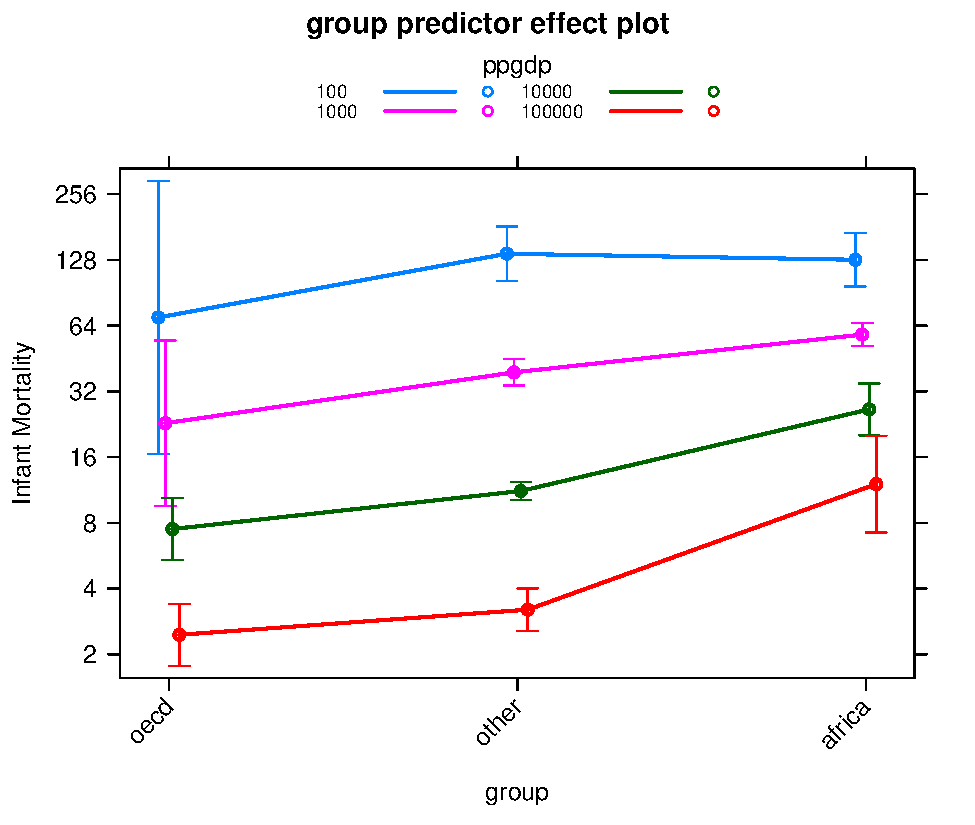
\includegraphics[width=0.49\textwidth]{fig3-a-1.pdf}
\includegraphics[width=0.49\textwidth]{fig3-b-1.pdf}
\caption{Predictor effect displays for the model for \code{infantMortality} fit to the \code{UN} data.\label{fig3}}
\end{figure}

The predictor effect displays are shown in Figure~\ref{fig3}.  The left panel has the focal predictor \code{group} on the horizontal axis.  The remaining predictor, the numeric predictor \code{ppgdp}, interacts with \code{group} and hence is evaluated at the supplied grid of four values equally spaced on the log scale, with a separate line drawn for each of the grid values of \code{ppdgp}.  Because \code{group} is a factor, $\yx{}$, which is equivalent to the linear predictor because the link function $\eta$ is the identity link, is computed only at the factor levels, indicated by the plotting symbols, which are slightly displaced horizontally to avoid overplotting.  The lines joining the plotting symbols are an aid for viewing the graph, and may be suppressed if desired.  We see that, in general, infant mortality at fixed levels of \code{ppgdp} is lowest in the \code{oecd} group and highest in \code{africa}; at the lowest level of \code{ppgdp}, however, fitted \code{infantMorality} is slightly lower in \code{africa} than in the \code{other} group, and the confidence interval for the \code{oecd} group is very wide, because there are no \code{oecd} countries at this level of \code{ppgdp}. In all three groups, infant mortality declines with \code{ppgdp}, though less so in \code{africa} than in the other groups.

The display in the right panel of Figure~\ref{fig3} is for the effect of \code{ppgdp}, with separate lines for the three groups of states overlaid on the same graph.  The lines are curved because \code{ppgdp} is represented by the regressor $\lvn{ppgdp}$ in the model. By default, a \emph{rug plot}, showing the marginal distribution of \code{ppgdp}, is shown at the bottom of the graph.  In this instance the inference is the same from the second plot as it is from the first, namely that infant mortality declines with per-capita GDP in all three groups, though less so in \code{africa} than in the other two groups, and that except at the lowest levels of \code{ppgdp}, infant mortality is lowest among the \code{oecd} states and highest in \code{africa} at fixed levels of \code{ppgdp},

\subsection{Term effects versus predictor effects}

Previous discussions of effect plots (such as \citealp{Fox87}), and previous versions of the \pkg{effects} package, develop what might be called high-order term effects, or, for short, \emph{term effects}: Term effect displays are drawn for combinations of predictors corresponding to the high-order terms in a model -- that is, terms that are not marginal to any terms in the model.

Consider, for example, the model formula \Rmod{y}{\aab{a}{b} +
  \aab{a}{c}}. We adopt the version of the \cite{WilkinsonRogers73}
notation for linear models that is used in \proglang{S} and
\proglang{R} \citep{ChambersHastie92}. In this notation, $\Rtilde{}$
separates the left- and right-hand sides of the model and \code{*} is
the crossing operator, and so, in expanded form, the model is
\Rmod{y}{1 + a + b + c + \acb{a}{b} + \acb{a}{c}}, where \code{y} is
the response, \code{1} represents the intercept, \code{a}, \code{b}
and \code{c} are the main effects of the three predictors, and
\code{\acb{a}{b}} and \code{\acb{a}{c}} are interactions. The
high-order terms in the model are \code{\acb{a}{b}} and
\code{\acb{a}{c}}.

The \code{allEffects} function applied to a model with this formula
produces two plots, one with \code{a} and \code{b} as the focal
predictors, and the other with \code{a} and {c} as the focal
predictors.  The \code{plot} method for more than one focal predictor
uses an algorithm to choose which predictor is plotted on the
horizontal axis and which is used as a conditioning variable. If the
formula has numeric predictors, then the left-most predictor in the
formula is used for the horizontal axis.

For example, if \code{b} were the only numeric predictor and \code{a} and \code{c} were factors, then the term effect plot for \code{\acb{a}{b}} would average over \code{c}, have \code{b} on the horizontal axis, and condition on \code{a}.  The term effect plot for \code{\acb{a}{c}} would average over \code{b}, and, for the horizontal axis, would use the factor with the fewest levels or the left-most factor if they have the same number of levels.

Neither of these plots corresponds to a predictor effect plot because they average over, rather than condition on, \code{c} in the first plot and \code{b} in the second plot, producing a display that is not invariant in shape with respect to the manner in which the levels of the factor \code{c} are averaged over in the term effect plot for \code{\acb{a}{b}}, or the typical value to which the numeric \code{b} is set in the term effect plot for \code{\acb{a}{c}}. In contrast, recall that averaging over or fixing the values of predictors in predictor effect plots affects only the height, and not the shape, of the effect. It is largely this invariance property that leads us to prefer predictor effects to term effects.

The most general function in the \pkg{effects} package is
\code{Effect}, in which the predictors in an effect are specified
explicitly. \code{Effect} may be used to produce both predictor and
term effect displays, including effect displays for terms that do not
appear in the model, such as an interaction higher-order term to those in
the model. For example, a plot equivalent to the predictor effect plot
for \code{b} could be obtained with the command
%
\begin{Schunk}
\begin{Sinput}
R> plot(Effect(c("a", "b", "c"), m), x.var = "b")
\end{Sinput}
\end{Schunk}
%
where \code{m} is the regression-model object.  This specification
recognizes that \code{b} interacts with both \code{a} and \code{c},
and the \code{x.var} argument overrides the default procedure for
determining the predictor on the horizontal axis of the graph.
Predictor effect plots for the other two predictors are obtained by
providing each predictor in turn as the \code{x.var} argument.

All predictor effect plots can be produced more conveniently using
%
\begin{Schunk}
\begin{Sinput}
R> plot(predictorEffects(m))
\end{Sinput}
\end{Schunk}
%
The three predictor effect plots in this example are views of the same
four-dimensional surface from three different view points. In the
preceding infant-mortality example, we used \code{predictorEffect} in
preference to \code{predictorEffects} to exert finer-grain control
over the resulting graphs.

\section{Partial residual plots}\label{sec-partial-residual-plots}

Whereas predictor effect plots are designed to summarize the conditional effects of each predictor given the others in a correctly specified regression model, partial residual plots are used to visualize misspecification of the mean function attributable to continuous predictors. We begin with a \emph{working model} given by (\ref{e1}) that is potentially misspecified. Suppose that $\x_i$ is the vector of predictors for the $i$th of $n$ observations in the data, and $y_i$ is the corresponding value of the response.  The \emph{estimated working linear predictor} for the $i$th observation is $h(\bbetahat, \x_i)$, and the corresponding \emph{working residuals} are $e(\x_i) = [y_i - \widehat{y}(\x_i)]\eta'(\x_i)$, where $\eta'(\x_i)$ is the first derivative of $\eta$ with respect to $\E(y|\x_i)$ \citep{CookCroos98}, which translates from the mean scale to the linear predictor scale.  Partial residual plots are always drawn in the linear predictor scale and only for numeric predictors.

Paralleling the development of predictor effect displays, for a numeric focal predictor $x_f$, we divide the $i$th vector of observed predictors into $\x_i = (x_{fi}, \x_{1i}, \x_{2i})$.  Partial residual plots are traditionally defined only when $\x_1 = \emptyset$.  In this case, the partial residual plot for a focal predictor $x_f$ is a graph of $n$ points, the $i$th of which is
\begin{equation}
 e(\x_i) + \left\{h[\bbetahat, (x_{fi}, \emptyset, \textbf{0})] - \betahat_0 \right\}  \textrm{ versus } \x_{fi} \label{e7}
\end{equation}
where $\emptyset$ has been inserted as a placeholder for the empty value of $\x_1$. The term in curly braces in (\ref{e7}) is called a \emph{partial regression function} and it represents the component of the fitted mean function that depends on $\x_{fi}$. The working residuals $e(\x_i)$ appear as random scatter around the partial regression function for a correctly specified model.

In certain circumstances, however, the scatter added by the residuals will be systematic. Suppose that in place of the working linear predictor in (\ref{e1}), the ``true'' linear predictor is
\begin{equation}
h(\bbeta, \x) +
          \left\{t(x_f) - h\left[\bbeta, (x_f, \emptyset, \mathbf{0})\right]\right\}  \label{e8}
\end{equation}
where $t(x_f)$ is a potentially nonlinear function of $x_f$.  If all the \emph{regressors} (not the \emph{predictors}) in $\x$ are at least approximately linearly related, and the  method used to estimate parameters is Fisher consistent, then a smoother fit to the partial residual plot for $x_f$ provides a visualization of $t$ \citep[Lemma 2.1]{Cook93} and possible misspecification with respect to $x_f$.  Extension from linear models to generalized linear models is provided by \citet{CookCroos98}.

Comparing (\ref{e7}) to (\ref{pe-1}), we can superimpose the partial residuals on the predictor effect plot simply by adding the constant $\betahat_0 + C$ to the abscissa of the points in (\ref{e7}).  The partial residuals are linearly translated, but nonlinear shapes, the main focus of the partial residuals, are unaffected.

When $\x_1 \neq \emptyset$, the predictor effect display consists of $G$ 2D line plots by conditioning on $\x_1^g$.  The points we add to the $g$th 2D plot are
\begin{equation}
e(\x_i) + h\left[\bbetahat, (x_{fi}, \x_{1i}, \x_2^a)\right] + C  \textrm{ versus } x_{f} \label{pe-4}
\end{equation}
for all $i$ such that $|\x_{1i} - \x_{1}^g|$ is minimized over $g$ for each element of $\x_{1}$, and the constant $C$ is chosen to match the intercept in the predictor effect display.   Cook's lemma can then be applied to each grid value separately to diagnose unmodelled curvature with respect to $x_f$ separately for each $g$.

\subsection{Example: Infant mortality revisited}\label{sec-infant-mortality-residuals}

Continuing with the UN infant mortality example in
Section~\ref{sec-preliminary-example}, we start with the response
variable \code{infantMortality} and predictor \code{ppgdp} unlogged.
The predictor effect plot for \code{ppgdp} with partial residuals is
shown in Figure~\ref{fig3a}. We initially leave Equatorial Guinea in
the data set.
%
\begin{Schunk}
\begin{Sinput}
R> m2 <- lm(infantMortality ~ group * ppgdp, data = UN)
R> plot(predictorEffects(m2, ~ ppgdp, partial.residuals = TRUE),
+    axes = list(x = list(rotate = 25), y = list(lim = c(0, 150))),
+    id = list(n = 1))
\end{Sinput}
\end{Schunk}
%
\begin{figure}[t!]
  \centerline{\includegraphics[width=1.0\textwidth]{fig3a-1.pdf}}
  \caption{Predictor effect plot with partial residuals for
    \code{ppgdp} when neither it nor the response
    \code{infantMortality} is log-transformed, labeling the most
    unusual point in each panel.\label{fig3a}}
\end{figure}

\begin{figure}[t!]
\centerline{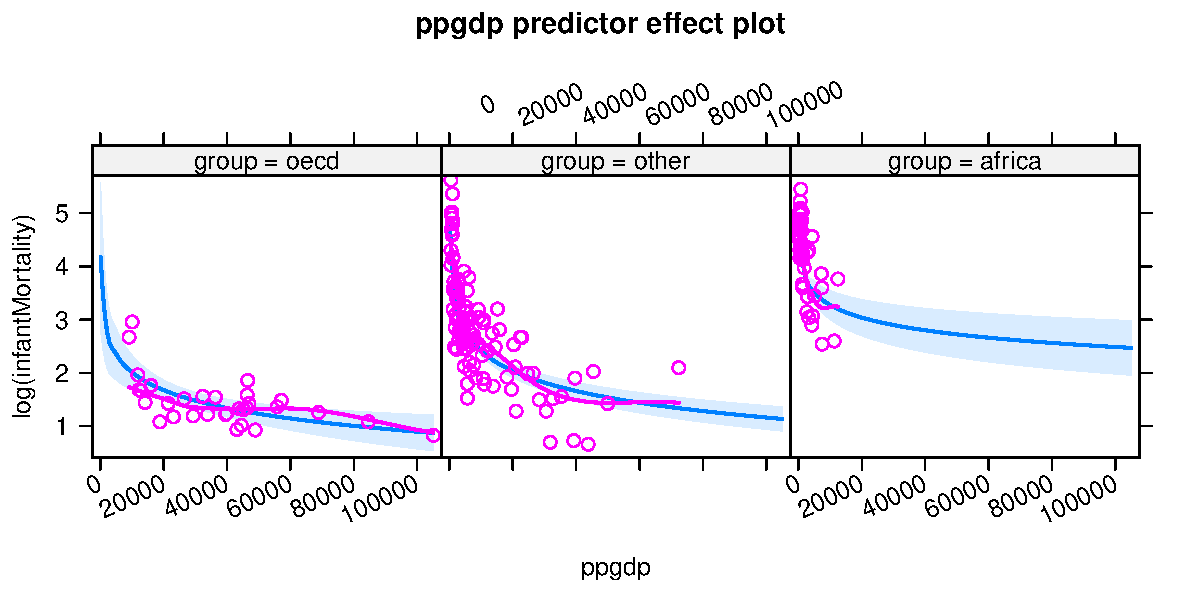
\includegraphics[width=1.0\textwidth]{fig3b-1.pdf}}
\caption{Predictor effect plot with partial residuals for \code{ppgdp} in the model with \code{ppgdp} and the response \code{infantMortality} log-transformed.\label{fig3b}}
\end{figure}

The \pkg{effects} package suppresses partial residuals for multi-line plots because of the confusion produced by overlapping residuals for different values of a conditioning predictor.  Instead, the residuals are plotted with the lines corresponding to different values of the conditioning predictors, here just the predictor \code{group}, in separate panels. The blue line in each panel represents the fitted model, with a point-wise 95-percent confidence band shown around the fitted effect. The magenta line in each panel is a \emph{loess nonparametric regression smooth} \citep{ClevelandGrosseShyu92}, using a span of 2/3 by default. The argument \code{id = list(n = 1)} to \code{plot} identifies the most unusual point in each panel, defined as the point with the largest Mahalanobis distance from the centroid of the points.

The points for \code{other} and \code{africa} are a clear mismatch for the fitted line, perhaps suggesting the log-transformations of \code{infantMortality} and \code{ppgdp} used in the initial example in Section~\ref{sec-preliminary-example}. The right-most point in \code{africa}, for Equatorial Guinea, is out of line with the rest of the African states, pairing a large value of \code{ppgdp} with a large value of \code{infantMortality}. The most unusual points in the other panels, Turkey in the \code{oecd} group and Afghanistan in the \code{other} group, are not out of line with the other points in their groups to the same degree. While extreme in their values of \code{ppgdp} and \code{infantMortality}, these two countries follow the general pattern of the data. Recall that we removed Equatorial Guinea, but not Turkey or Afghanistan, in the model fit in Section~\ref{sec-preliminary-example}.

The partial residuals have the added benefit of highlighting that while \code{ppgdp} is both relatively high and highly variable in the \code{oecd} group, it has relatively small variation in \code{africa}, where it is concentrated in very low values.  The \code{other} group is intermediate.  When both the response variable and \code{ppgdp} are log-transformed, as in model \code{m1} in Section~\ref{sec-preliminary-example}, the partial-residual plots are much more satisfactory (see~Figure~\ref{fig3b}):
%
\begin{Schunk}
\begin{Sinput}
R> plot(predictorEffects(m1, ~ ppgdp, partial.residuals = TRUE),
+    axes = list(x = list(rotate = 25)))
\end{Sinput}
\end{Schunk}

\subsection{Conditioning on continuous predictors}

When $\x_1$ includes continuous numeric predictors, as in the first example in the next section, the assignment of partial residuals to one of the grid of conditioning values introduces additional variation, because the linear predictor is evaluated at $(x_{fi}, \x_{1i}, \x_{2}^a)$ rather than at the grid value $(x_{fi}, \x_{1}^g, \x_{2}^a)$.  That is, there is a potential extra source of variability in the plot due to conditioning.  If we assume that the value of this difference has a symmetric distribution about zero, then, from \citet[Lemma 2.1]{Cook93}, the  \emph{unadjusted partial residual plot} (\ref{pe-4}) visualizes  $t(x_f)$ with extra variation. If the difference is \emph{not} symmetrically distributed, as is likely, for example, for extreme values of the continuous predictors in $\x_1$, then bias may be introduced.

A predictor effect display in linear predictor scale with \emph{partial residuals adjusted for conditioning} includes the points given for the $g$th plot by
\begin{equation}
e(\x_i) + h\left[\bbetahat, (x_{fi}, \x_{1}^g, \x_2^a)\right] + C  \textrm{ versus } x_{f} \label{pe-5}
\end{equation}
substituting the grid values $\x_{1}^g$ for the data values $\x_{1i}$ of the conditioning predictors. This plot also visualizes $t(x_f)$ for each $g$ under the same conditions as the unadjusted version, but the visualization may be sharper. The adjusted version is implemented in the \pkg{effects} package.

The requirement of linearly related regressors for the usefulness of partial residual plots may be restrictive on its face, particularly in problems with $\x_1 \neq \emptyset$.  Because we are conditioning on $\x_1 = \x_1^g$, however, linearly related regressors are only required within a fixed value of $\x_1$. Moreover, experience suggests that only fairly strong nonlinear relationships among the regressors prove to be problematic.

\section{More examples}\label{sec-examples}

\subsection{Volunteering for a psychological experiment}

\citet{CowlesDavis87} conducted a study on volunteering for a
psychological experiment, in which the subjects were students in an
introductory psychology course. The authors of the study collected
data on the students' gender, on the personality dimensions
extraversion and neuroticism, each of which ranges potentially from
zero to 24, and on the students' willingness to volunteer for an
experiment. Of the 1421 students for whom data were collected, 597
were willing to serve as volunteers. The data are in the \code{Cowles}
data frame in the \pkg{carData} package:
%
\begin{Schunk}
\begin{Sinput}
R> summary(Cowles)
\end{Sinput}
\begin{Soutput}
  neuroticism     extraversion       sex      volunteer
 Min.   : 0.00   Min.   : 2.00   female:780   no :824  
 1st Qu.: 8.00   1st Qu.:10.00   male  :641   yes:597  
 Median :11.00   Median :13.00                         
 Mean   :11.47   Mean   :12.37                         
 3rd Qu.:15.00   3rd Qu.:15.00                         
 Max.   :24.00   Max.   :23.00                         
\end{Soutput}
\end{Schunk}
%
Cowles and Davis expected extraversion and neuroticism to interact in affecting volunteering, leading to the following logistic regression model:
%
\begin{Schunk}
\begin{Sinput}
R> library("car")
R> mod.cowles.1 <- glm(volunteer ~ sex + neuroticism * extraversion,
+    data = Cowles, family = binomial)
R> summary(mod.cowles.1)
\end{Sinput}
\begin{Soutput}
Call:
glm(formula = volunteer ~ sex + neuroticism * extraversion, family = binomial, 
    data = Cowles)

Deviance Residuals: 
    Min       1Q   Median       3Q      Max  
-1.4749  -1.0602  -0.8934   1.2609   1.9978  

Coefficients:
                          Estimate Std. Error z value   Pr(>|z|)
(Intercept)              -2.358207   0.501320  -4.704 0.00000255
sexmale                  -0.247152   0.111631  -2.214    0.02683
neuroticism               0.110777   0.037648   2.942    0.00326
extraversion              0.166816   0.037719   4.423 0.00000975
neuroticism:extraversion -0.008552   0.002934  -2.915    0.00355

(Dispersion parameter for binomial family taken to be 1)

    Null deviance: 1933.5  on 1420  degrees of freedom
Residual deviance: 1897.4  on 1416  degrees of freedom
AIC: 1907.4

Number of Fisher Scoring iterations: 4
\end{Soutput}
\begin{Sinput}
R> Anova(mod.cowles.1)
\end{Sinput}
\begin{Soutput}
Analysis of Deviance Table (Type II tests)

Response: volunteer
                         LR Chisq Df  Pr(>Chisq)
sex                        4.9184  1    0.026572
neuroticism                0.3139  1    0.575316
extraversion              22.1372  1 0.000002538
neuroticism:extraversion   8.6213  1    0.003323
\end{Soutput}
\end{Schunk}
%
We use the \code{Anova} function in the \pkg{car} package
\citep{FoxWeisberg11} to obtain Type II tests for the terms in the
model.  As expected, the interaction between \code{neuroticism} and
\code{extraversion} has a small $p$~value, and some evidence for a
difference between the sexes is also apparent.

The predictor effect displays in mean scale (i.e., the probability
scale) can all be drawn simultaneously by the \code{predictorEffects}
function, as shown in Figure~\ref{new-cowles-1}:
%
\begin{Schunk}
\begin{Sinput}
R> plot(predictorEffects(mod.cowles.1,
+    xlevels = list(extraversion = seq(0, 24, by = 6),
+    neuroticism = seq(0, 24, by = 6))),
+    axes = list(y = list(type = "response")),
+    lines = list(multiline = TRUE), rows = 1, cols = 3)
\end{Sinput}
\end{Schunk}
%
\begin{figure}[t!]
  \centering
    \includegraphics[width=\textwidth]{new-cowles-1-1.pdf}
  \caption{Predictor effect displays for Cowles and Davis's logistic regression for volunteering for a psychological experiment.}\label{new-cowles-1}
\end{figure}
The lines in the predictor effect plots for \code{neuroticism} and \code{extroversion} are not straight because of the conversion from linear predictor (logit) to mean (probability) scale, obtained by specifying the argument \code{axes = list(y = list(type = "response"))} to \code{plot}. As before, we obtain multi-line plots for the continuous predictors by \code{lines = list(multiline = TRUE)}. We use the \code{xlevels} argument to \code{predictorEffects} to exert control over the values of these predictors. The \code{rows} and \code{cols} arguments to \code{plot} specify that the meta-array of effect displays should be arranged horizontally.  By default, confidence intervals around the estimated effects are suppressed in multi-line plots; as before, they could be turned on by \code{confint = list(style = "auto")}. The \code{predictorEffects} function can also be used for a subset of predictors; see the function's help page.

The effect plot for \code{sex} is little more than a visualization of the regression coefficient for this factor, with females somewhat more likely than males to volunteer, and because the difference in estimated probabilities is small, the change to mean scale suggests that this visualization would apply for any meaningful averaging over the remaining predictors.  The other two displays are two views of the same 3D surface, because both have $\x_2 = (\mbox{\code{sex}})$ fixed in the same way.  The second display suggests clearly that as \code{neuroticism} increases, the probability of volunteering increases for subjects with low \code{extraversion}, but decreases for subjects with high \code{extraversion}.  The third display, with \code{extraversion} on the horizontal axis, shows that the probability of volunteering generally increases with \code{extraversion}, at a very high rate when \code{extraversion} is low, and a much lower rate when \code{neuroticism} is high; at the highest level of \code{neuroticism}, the relationship becomes negative.  In this instance, both displays of the interactions can be useful, as they emphasize somewhat different stories.

Figure~\ref{new-cowles-2} is the predictor effect plot for \code{neuroticism} in linear predictor (logit) scale with the partial residuals shown:
%
\begin{Schunk}
\begin{Sinput}
R> plot(predictorEffects(mod.cowles.1, ~ neuroticism, 
+    partial.residuals = TRUE), lattice = list(layout = c(4, 1)))
\end{Sinput}
\end{Schunk}
%
\begin{figure}[t!]
  \centering
    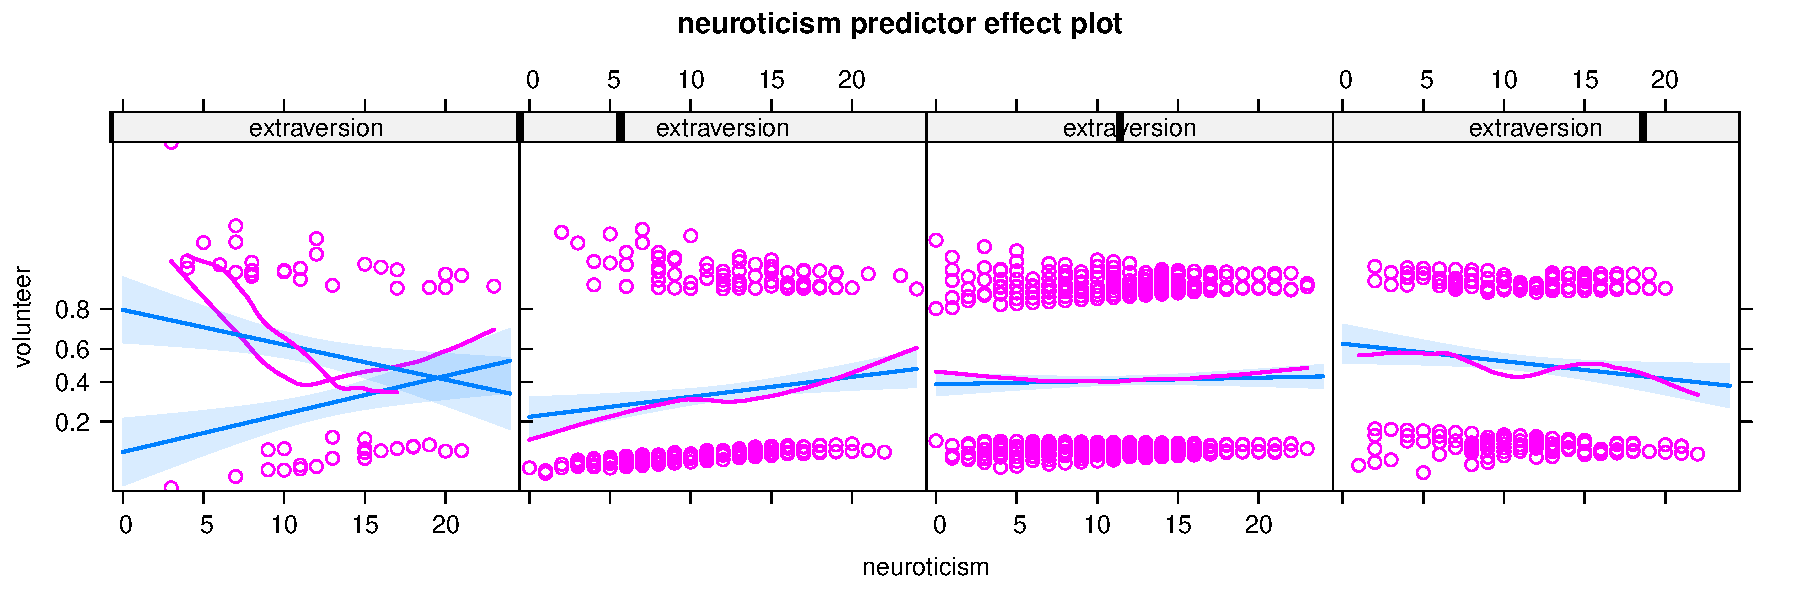
\includegraphics[width=\textwidth]{new-cowles-2-1.pdf}
  \caption{Predictor effect display for \code{neuroticism} showing partial residuals.}\label{new-cowles-2}
\end{figure}
The \code{lattice} argument to \code{plot} sets the \pkg{lattice} package \code{layout} argument, producing a plot with four panels arranged in one row (with the unusual column, row order standard for the \pkg{lattice} \code{layout} argument). The conditionally fixed values of \code{extraversion} increase from left to right across the range of this predictor, as indicated by the black line in the strip at the top of each panel.

For this logistic regression, the vertical axis is on the logit scale,
and the default in the \pkg{effects} package is to label tick-marks on
this axis with values of the inverse link function applied to the
logits -- that is, with corresponding probabilities. Because this is a
diagnostic plot, we have not bothered to customize the location of the
tick-marks on the vertical axis. The partial residuals are given by
the magenta open circles, and the magenta line is the loess smooth of
the partial residuals, with default span of 2/3. As before, the blue
lines, which are straight on the logit scale, represent the fitted
model, with the 95-percent point-wise confidence envelope around the
fit superimposed.  Robust smooths for non-Gaussian generalized linear
models can result in substantial bias in the fitted curve
\citep{LandwehrPregibonShoemaker80}, and so a non-robust loess
smoother is used. The general agreement of the smooths with the fitted
effect suggests that the model reasonably represents the data.

As an additional check, we fit an alternative model to Cowles and
Davis's data, in which each of \code{neuroticism} and
\code{extraversion} is represented by a five-degree-of-freedom natural
regression spline. The resulting model uses 25 degrees of freedom for
the interaction, along with five degrees of freedom for each of the
neuroticism and extraversion main effects, and is consequently much
more flexible than the original model with a linear-by-linear
interaction. A likelihood-ratio test comparing the new model to the
original one fails to reveal significant lack of fit in the original
model, and the original model is strongly preferred by both the AIC
and BIC:
%
\begin{Schunk}
\begin{Sinput}
R> library("splines")
R> mod.cowles.2 <- glm(volunteer ~ sex + ns(neuroticism, 5) * 
+    ns(extraversion, 5), data = Cowles, family = binomial)
R> anova(mod.cowles.1, mod.cowles.2, test = "Chisq")
\end{Sinput}
\begin{Soutput}
Analysis of Deviance Table

Model 1: volunteer ~ sex + neuroticism * extraversion
Model 2: volunteer ~ sex + ns(neuroticism, 5) * ns(extraversion, 5)
  Resid. Df Resid. Dev Df Deviance Pr(>Chi)
1      1416     1897.4                     
2      1384     1857.0 32   40.468   0.1448
\end{Soutput}
\begin{Sinput}
R> cbind(AIC(mod.cowles.1, mod.cowles.2), BIC(mod.cowles.1, mod.cowles.2))
\end{Sinput}
\begin{Soutput}
             df      AIC df      BIC
mod.cowles.1  5 1907.440  5 1933.736
mod.cowles.2 37 1930.972 37 2125.560
\end{Soutput}
\end{Schunk}
%
\subsection{Canadian occupational prestige data}\label{sec-prestige-data}

\citet{BlishenMcRoberts76} assembled data on the prestige, income
level, and education level of males in 102 Canadian occupations, with
the purpose of developing a prediction equation for occupational
prestige based on income and education. We analyze similar data here,
although the income and education scores in our data set are for
\emph{all} occupational incumbents, rather than just for men. These
data were also analyzed by \citet{FoxSuschnigg89}. The prestige scores
are average ratings for the occupations in a national survey conducted
in the mid-1960s \citep{PineoPorter67}. The income and education
scores are averages from the 1971 Canadian census. We classified 98 of
the occupations by type: blue collar, white collar, and professional
or managerial. Four of the occupations -- ``athletes,'' ``newsboys,''
``babysitters,'' and ``farmers'' -- did not fit into this
classification and are dropped from our analysis. The Canadian
occupational prestige data are in the data frame \code{Prestige} in
the \pkg{carData} package:
%
\begin{Schunk}
\begin{Sinput}
R> summary(Prestige)
\end{Sinput}
\begin{Soutput}
   education          income          women           prestige    
 Min.   : 6.380   Min.   :  611   Min.   : 0.000   Min.   :14.80  
 1st Qu.: 8.445   1st Qu.: 4106   1st Qu.: 3.592   1st Qu.:35.23  
 Median :10.540   Median : 5930   Median :13.600   Median :43.60  
 Mean   :10.738   Mean   : 6798   Mean   :28.979   Mean   :46.83  
 3rd Qu.:12.648   3rd Qu.: 8187   3rd Qu.:52.203   3rd Qu.:59.27  
 Max.   :15.970   Max.   :25879   Max.   :97.510   Max.   :87.20  
     census       type   
 Min.   :1113   bc  :44  
 1st Qu.:3120   prof:31  
 Median :5135   wc  :23  
 Mean   :5402   NA's: 4  
 3rd Qu.:8312            
 Max.   :9517            
\end{Soutput}
\end{Schunk}
%
Similar to the analysis by Blishen and McRoberts, we will begin by
fitting an additive linear model with continuous numeric predictors
\code{income} and \code{education}, and factor predictor
\code{type}. Blishen and McRoberts's original analysis did not,
however, include the predictor \code{type}. We reorder the levels of
\code{type} from their default alphabetical ordering to their natural
ordering:
%
\begin{Schunk}
\begin{Sinput}
R> Prestige$type <- factor(Prestige$type, levels = c("bc", "wc", "prof"))
R> mod.prestige.1 <- lm(prestige ~ income + education + type,
+    data = Prestige)
R> summary(mod.prestige.1)
\end{Sinput}
\begin{Soutput}
Call:
lm(formula = prestige ~ income + education + type, data = Prestige)

Residuals:
     Min       1Q   Median       3Q      Max 
-14.9529  -4.4486   0.1678   5.0566  18.6320 

Coefficients:
              Estimate Std. Error t value    Pr(>|t|)
(Intercept) -0.6229292  5.2275255  -0.119       0.905
income       0.0010132  0.0002209   4.586 0.000014049
education    3.6731661  0.6405016   5.735 0.000000121
typewc      -2.7372307  2.5139324  -1.089       0.279
typeprof     6.0389707  3.8668551   1.562       0.122

Residual standard error: 7.095 on 93 degrees of freedom
  (4 observations deleted due to missingness)
Multiple R-squared:  0.8349,	Adjusted R-squared:  0.8278 
F-statistic: 117.5 on 4 and 93 DF,  p-value: < 2.2e-16
\end{Soutput}
\begin{Sinput}
R> Anova(mod.prestige.1)
\end{Sinput}
\begin{Soutput}
Anova Table (Type II tests)

Response: prestige
          Sum Sq Df F value       Pr(>F)
income    1058.8  1 21.0339 0.0000140492
education 1655.5  1 32.8882 0.0000001205
type       591.2  2  5.8721     0.003966
Residuals 4681.3 93                     
\end{Soutput}
\end{Schunk}
%
The ANOVA table for the model reveals that all three terms have very
small $p$~values, suggesting that all three predictors may be useful.

An effect plot with partial residuals for \code{income} in this
additive model is, except for the scaling of the vertical axis, a
traditional partial residual plot:
%
\begin{Schunk}
\begin{Sinput}
R> plot(predictorEffects(mod.prestige.1, ~ income,
+    partial.residuals = TRUE))
\end{Sinput}
\end{Schunk}
%
The resulting graph, shown in Figure~\ref{fig-prestige-1}, reveals apparent nonlinearity in the partial regression of \code{prestige} on \code{income}.

\begin{figure}[t!]
  \centering
    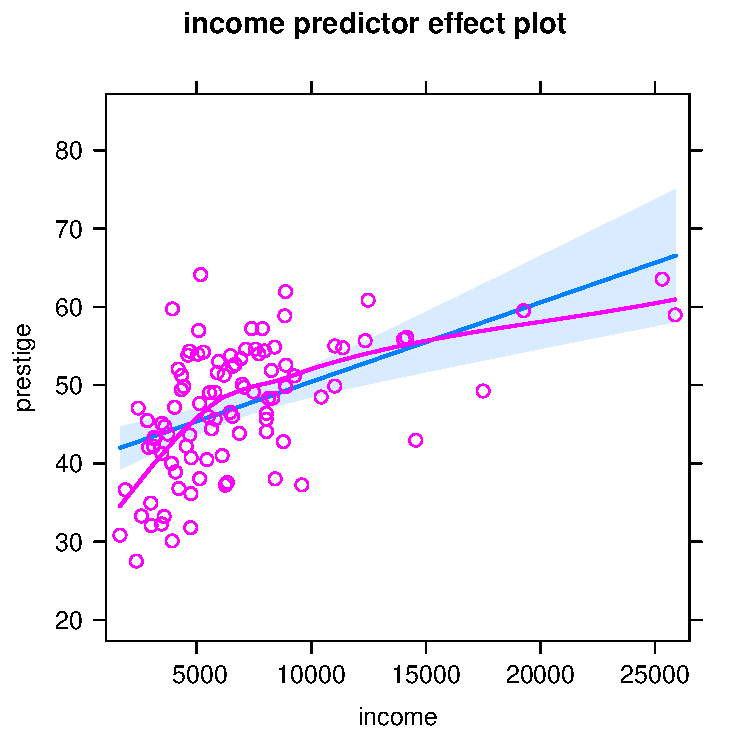
\includegraphics[width=0.5\textwidth, trim = 0 10 0 5, clip]{fig-prestige-1-1.pdf}
    \caption{Predictor effect display with partial residuals for
      \code{income} in the additive regression of \code{prestige} on
      \code{income}, \code{education}, and \code{type} of
      occupation.}\label{fig-prestige-1}
\end{figure}

An alternative story, however, is told by the term effect plot for
\code{income} and \code{type} of occupation, which is higher-order
than the terms actually in the model, and which can be computed using
the \code{Effect} function in the \pkg{effects} package, producing
Figure~\ref{fig-prestige-2}:
%
\begin{Schunk}
\begin{Sinput}
R> plot(Effect(c("income", "type"), mod.prestige.1,
+    partial.residuals = TRUE), partial.residuals = list(span = 0.9),
+    axes = list(x = list(rotate = 25)), lattice = list(layout = c(3, 1)))
\end{Sinput}
\end{Schunk}
%
\begin{figure}[t!]
  \centering
    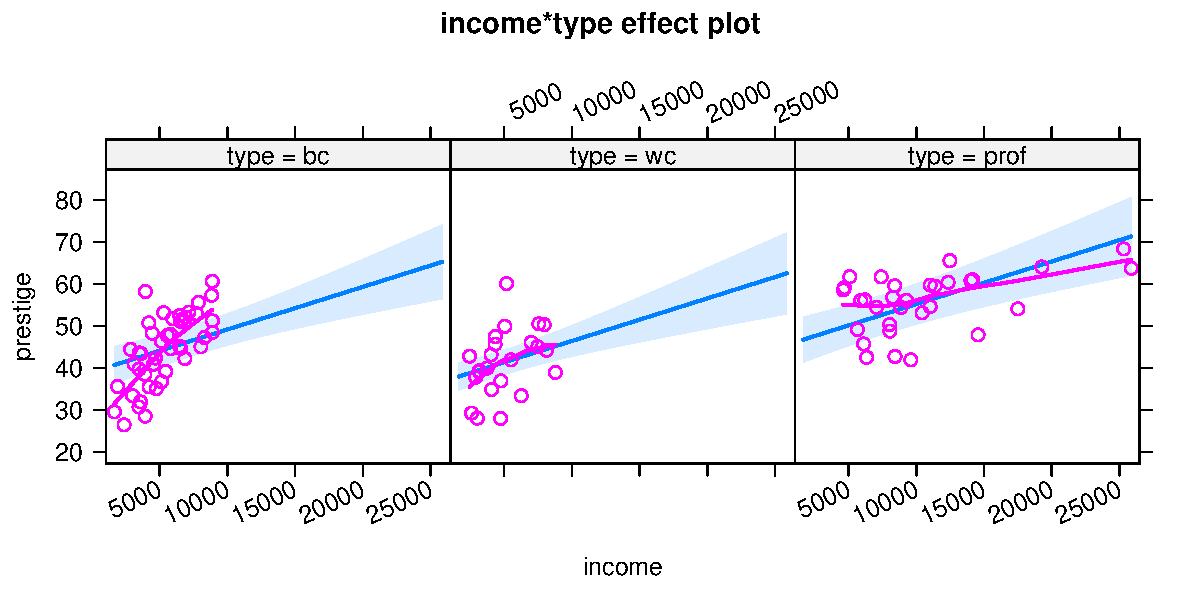
\includegraphics[width=\textwidth, trim = 0 10 0 5, clip]{fig-prestige-2-1.pdf}
  \caption{Term effect display with partial residuals for the
    predictors \code{income} and \code{type} in the additive
    regression of \code{prestige} on \code{income}, \code{education},
    and \code{type} of occupation.}\label{fig-prestige-2}
\end{figure}
We use a large span of 0.9 for the loess smoothers in this graph
because dividing the data by the levels of the factor \code{type}
leaves relatively few cases in each panel of the graph. Although the
relationship between \code{prestige} and \code{income} in each panel
appears positive and reasonably linear, the assumption that the slopes
are equal in the panels is questionable, with an apparently larger
slope for blue-collar occupations, a smaller slope for professional
and managerial occupations, and an intermediate slope for white-collar
occupations.

Adding the linear \code{income}-by-\code{type} interaction to the
model, as suggested by Figure~\ref{fig-prestige-2}, confirms this
impression:
%
\begin{Schunk}
\begin{Sinput}
R> mod.prestige.2 <- lm(prestige ~ type * income + education,
+    data = Prestige)
R> anova(mod.prestige.1, mod.prestige.2)
\end{Sinput}
\begin{Soutput}
Analysis of Variance Table

Model 1: prestige ~ income + education + type
Model 2: prestige ~ type * income + education
  Res.Df    RSS Df Sum of Sq      F     Pr(>F)
1     93 4681.3                               
2     91 3791.3  2    890.02 10.681 0.00006809
\end{Soutput}
\end{Schunk}
%
Of course, the test for the interaction needs to be taken with a grain
of salt, in that we added the interaction to the model after examining
the data.

Figure~\ref{fig-prestige-3} is the term effect plot for \code{income}
and \code{type} (equivalent to the predictor effect plot for
\code{income}) in the model that includes the income-by-type
interaction:
%
\begin{Schunk}
\begin{Sinput}
R> plot(Effect(c("income", "type"), mod.prestige.2,
+    partial.residuals = TRUE), partial.residuals = list(span = 0.9),
+    axes = list(x = list(rotate = 25)), lattice = list(layout = c(3, 1)))
\end{Sinput}
\end{Schunk}
%
\begin{figure}[t!]
  \centering
    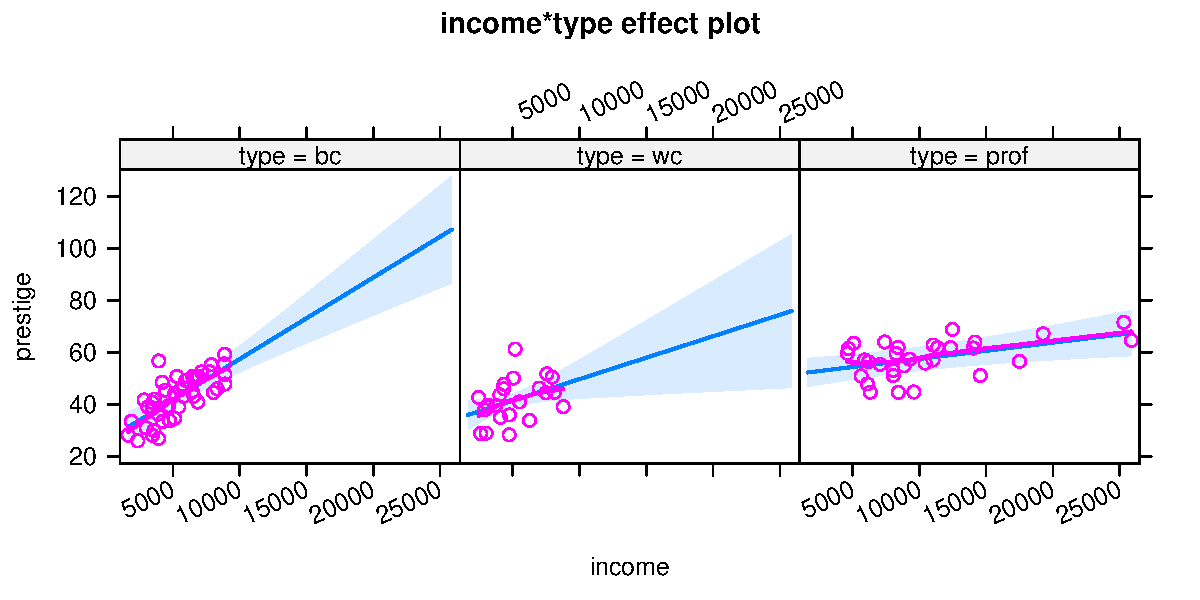
\includegraphics[width=\textwidth, trim = 0 10 0 5, clip]{fig-prestige-3-1.pdf}
  \caption{Term effect display with partial residuals for
    \code{income} and \code{type} in the model incorporating the
    \code{\acb{income}{type}} interaction.}\label{fig-prestige-3}
\end{figure}
The nonlinearity apparent in the partial residual plot for \code{income} in the additive model in Figure~\ref{fig-prestige-1} was induced by the relationship between \code{income} and occupational \code{type}, together with the unmodelled \code{income}-by-\code{type} interaction: Blue-collar occupations, for which the \code{income} slope is steep, are clustered at lower incomes, while professional occupations, for which the \code{income} slope is smaller, tend to have higher incomes. In addition to supporting the respecified regression, Figure~\ref{fig-prestige-3} makes a useful pedagogical point about precision of estimation of the regression surface: The confidence envelopes show that the fitted regression is sensibly imprecisely estimated where there are no data.

\pagebreak

\subsection{Contrived regression data}\label{sec-contrived-data}

We will analyze contrived data generated according to the following setup:

\begin{itemize}

\item We sample $n = 5000$ observations from a trivariate distribution for predictors $x_1$, $x_2$, and $x_3$, with uniform margins on the interval $[-2, 2]$, and with a prespecified bivariate correlation $\rho$ between each pair of predictors. The method employed, described by \citet{Schumann15} and traceable to results reported by \citet{Pearson07}, produces predictors that are nearly linearly related. Using 5000 observations allows us to focus on essentially asymptotic behavior of partial residuals in effect plots while still being able to discern individual points in the resulting graphs.

\item We then generate the response $y$ according to the model
\begin{equation}
y = \beta_0 + h\left(\bbeta, \{x_1, x_2, x_3\}\right) + \varepsilon
\end{equation}
where $\varepsilon \sim \N(0, 1.5^2)$. The regression function $h(\cdot)$ varies from example to example.

\end{itemize}
%
A variety of contrived examples generated in this manner, along with \R{} functions for flexibly generating simulated data, are included in a vignette in the \pkg{effects} package.


\begin{figure}[t!]
  \centering
    \includegraphics[width=1\textwidth]{fig-contrived-4a-1.pdf}
  \caption{Effect displays with partial residuals for the predictors $x_1$, $x_2$, and $x_3$ in the incorrect model $y \captilde x_1 + x_2 + x_3$ fit to data generated with the mean function $\E(y|\x) = x_1^2 + x_2x_3$, with moderately correlated predictors.}\label{fig-contrived-4a}
\end{figure}
\begin{figure}[t!]
  \centering
    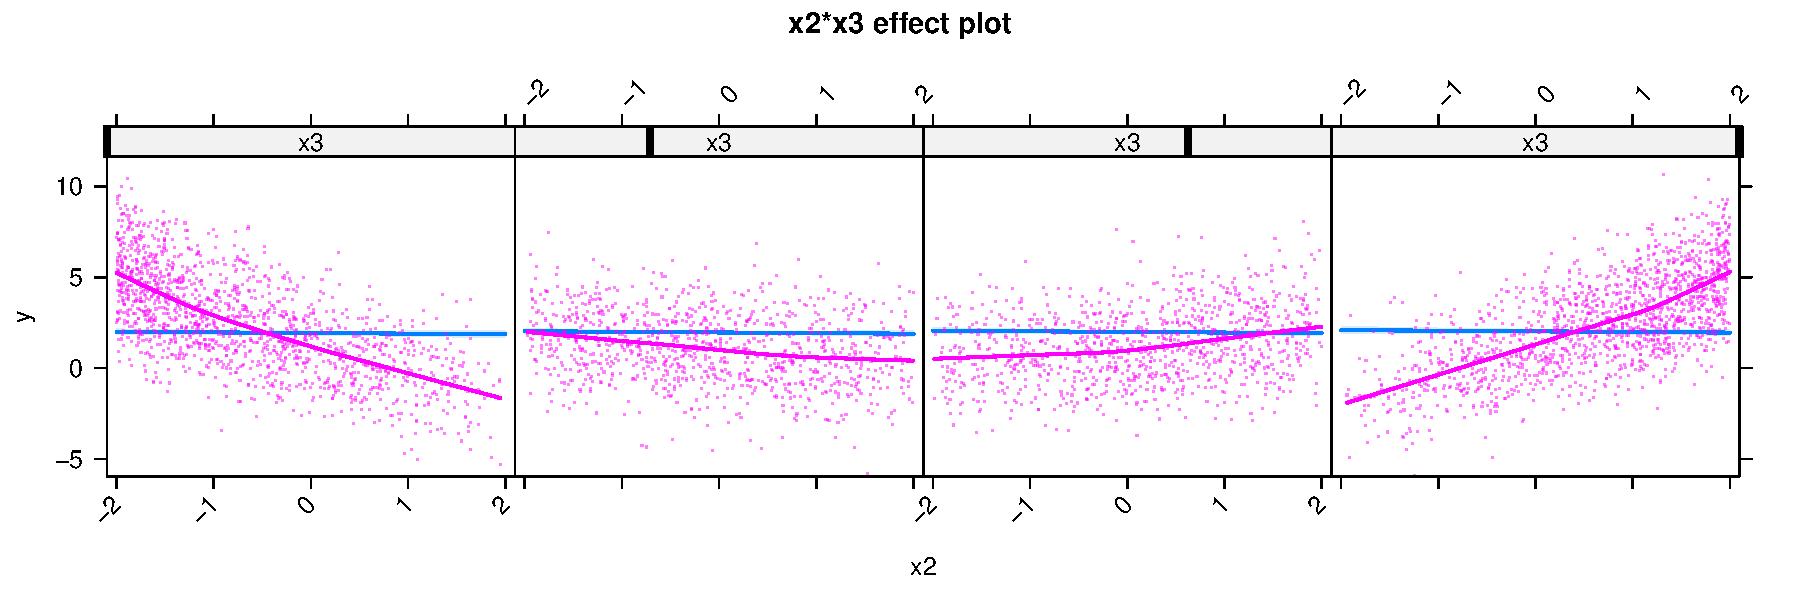
\includegraphics[width=1\textwidth]{fig-contrived-4b-1.pdf} \\
    \includegraphics[width=1\textwidth]{fig-contrived-4c-1.pdf}
  \caption{Term effect displays with partial residuals for $\{x_2, x_3 \}$ (top) and for $\{x_1, x_2 \}$ (bottom), the first of which corresponds to the missing \inter{x_2}{x_3} interaction in the model generating the data.}\label{fig-contrived-4b}
\end{figure}


In a sense, the example developed in this section and the examples in
the vignette are unnecessary, because the results obtained are
generally predictable from Cook's theoretical analysis of
partial-residual plots, discussed in
Section~\ref{sec-partial-residual-plots}. We nevertheless think that
these examples are useful for illustrating the application of Cook's
analysis to partial-residual effect plots and for cultivating judgment
about how to interpret these plots.

\begin{figure}[t!]
  \centering
    \includegraphics[width=0.45\textwidth]{fig-contrived-5a-1.pdf} \\
    \includegraphics[width=0.9\textwidth]{fig-contrived-5b-1.pdf}  \\
    \includegraphics[width=0.9\textwidth]{fig-contrived-5c-1.pdf}
  \caption{Effect displays with partial residuals for $x_1$ and $\{x_2, x_3 \}$, which correspond to the terms in the model generating \emph{and} fitted to the data, $y \Rtilde{} x_1^2 + x_2 * x_3$, and for $\{x_1, x_2 \}$, which corresponds to an interaction that is not in the model.}\label{fig-contrived-5}
\end{figure}
%\end{contrived}

We consider a true model that combines nonlinearity and interaction,
$\E(y|\x) = x_1^2 + x_2 x_3$; the predictors are moderately
correlated, with $\rho = 0.5$. We then fit the incorrect working model
$y \Rtilde x_1 + x_2 + x_3$ to the data, producing the predictor
effect displays with partial residuals in
Figure~\ref{fig-contrived-4a}, for the predictors $x_1$, $x_2$, and
$x_3$, which appear additively in the working model, and the term
effect displays in Figure~\ref{fig-contrived-4b} for $\{x_2, x_3 \}$
and $\{x_1, x_2 \}$, corresponding respectively to the incorrectly
excluded \inter{x_2}{x_3} term and the correctly excluded
\inter{x_1}{x_2} interaction.

The nonlinearity in the partial relationship of $y$ to $x_1$ shows up
clearly. The nonlinearity apparent in the plots for $x_2$ and $x_3$ is
partly due to contamination with $x_1$, but largely to the unmodelled
interaction between $x_2$ and $x_3$, coupled with the correlation
between these predictors. A similar phenomenon was noted in our
analysis of the Canadian occupational prestige data in
Section~\ref{sec-prestige-data}, where the unmodelled interaction
between \code{type} and \code{income} induced nonlinearity in the
partial relationship of \code{prestige} to \code{income}. The plot
corresponding to the missing \inter{x_2}{x_3} term (in the top panel
of Figure~\ref{fig-contrived-4b}) does a good job of detecting the
unmodelled interaction, and curvature in this plot is slight. The plot
for the \inter{x_1}{x_2} term (in the bottom panel of
Figure~\ref{fig-contrived-4b}), a term neither in the true model nor
in the working model, primarily reveals the unmodelled nonlinearity in
the partial relationship of $y$ to $x_1$.

If we fit the correct model, $y \Rtilde{} x_1^2 + x_2 * x_3$, to the
data, we obtain the plots shown in Figure~\ref{fig-contrived-5}. As
theory suggests, the partial residuals in these effect displays
validate the model, supporting the exclusion of the \inter{x_1}{x_2}
interaction, the linear-by-linear interaction between $x_2$ and $x_3$,
and the quadratic partial relationship of $y$ to $x_1$.

\section{Discussion}\label{sec-discussion}

Graphical methods play a central role in many aspects of statistical
data analysis.  Their use roughly divides into three phases: an
\emph{exploratory phase}, in which an analyst examines data
graphically for expected and unexpected structure \citep{Tukey77}; an
\emph{analysis phase}, in which graphs are used as an aid in
formulating and assessing the adequacy of statistical models fit to
the data; and a \emph{presentation phase}, in which graphs provide
summaries of an analysis that may be shared with others.  Predictor
effect plots are straightforward summary graphs for each predictor in
a regression model.  These plots are analogous to the usual numeric
summaries of a fitted model, providing a separate explanation of the
role of each predictor in a regression model after conditioning on all
other relevant predictors.

The contribution of this article and the associated software in the \pkg{effects} package is two-fold:
\begin{enumerate}

\item We introduce predictor effect displays as an alternative to term effect displays. Predictor effect displays correspond more naturally to how researchers interpret the results of complex regression models, are simpler to describe formally, and have improved invariance properties relative to term effect displays.

\item Although effect displays, including effect plots with partial residuals, are related to other approaches for interpreting complex regression models, and although the general scheme employed using two-dimensional conditioning plots is not entirely original (see below for both of these points), the conceptualization described in this paper and its implementation in the \pkg{effects} package are novel in certain respects and more general than alternative approaches.

\end{enumerate}

Partial residuals in effect plots can help to detect incorrectly
specified models and point toward their improvement. If the model is
correctly specified, then partial residuals for predictor effects, for
the high-order terms of the model, and for effects of higher-order to
those included in the model, should confirm the correctness of the
model. On the other hand, if the model is incorrectly specified, then
partial residual plots should not be interpreted na\"{i}vely, because
a failure in one part of the model can contaminate plots for other
combinations of predictors. For example, as we have shown, failure to
model an interaction can appear as nonlinearity in a partial residual
plot for one of the predictors entering the unmodelled interaction;
and unmodelled nonlinearity in one predictor can also appear in the
partial residuals for other predictors that are correlated with
it. Awareness of these potential artifacts increases the utility of
partial-residual effect plots in improving complex regression
models. For example, if multiple issues are detected in partial
residual plots, it is generally sensible to address them one at a
time, rechecking at each step.

Displays similar to effect plots are also available in a number of other implementations.
\begin{itemize}

\item In \proglang{R}, the \pkg{visreg} \citep{visreg} package is most
  similar to \pkg{effects}, but it provides only for conditioning on
  \emph{specific levels} of a factor rather than \emph{averaging over}
  them, as is done in the \pkg{effects} package.  The \pkg{visreg}
  package also seems to be limited to two-factor interactions,
  excluding the possibility of plotting higher-order terms, so
  problems with more than one interaction may not be properly
  displayed.

\item The \code{margins} and \code{marginsplot} programs in
  \proglang{Stata} \citep{Stata15} create displays that are similar to
  effect plots, except averaging or conditioning is over the empirical
  distribution of the regressors rather than the predictors, which can
  lead to invariance problems.  As far was we can see, partial
  residuals cannot be added to a margins plot.

\item Least-squares means, a generalization of adjusted means in
  analysis of covariance, introduced by \citealp{Fisher36}, as
  implemented in \proglang{SAS} \citep{sas12} and the \pkg{lsmeans}
  package for \R{} \citep{Lenth16, LenthHerve15}, are capable of
  displaying interactions among factors, and in certain instances
  least-squares means coincide with effect displays. Partial residuals
  are not relevant to displays of least-squares means, however. The 
  \pkg{lsmeans} has been superceeded by the \pkg{emmeans} package 
  \citep{lenth18}.
\end{itemize}

For a linear predictor with only main effects, adding partial
residuals to an effect plot is straightforward, and provides little
that is new.  For example, the plots produced by the \code{gam}
functions in the \pkg{mgcv} \citep{Wood17} and \pkg{gam} \citep{gam}
packages are effect plots with partial residuals added. In an early
general article on Trellis displays, \cite{becker96} include a graph
(their Figure~6) that they describe as a partial residual plot. Rather
than fitting an explicit model to the data, however, they subtract
marginal means for one factor from the data in a three-way
classification with one case per cell, and then plot the resulting
values against the other two factors. This procedure works because the
data are balanced, and is equivalent to fitting a one-way ANOVA for
one of the three factors. The procedure is not general, however, and
the plotted values would not typically be termed partial residuals.

The functions in the \pkg{effects} package rely on the presence of a
linear predictor in a regression model, and are therefore not suitable
for less structured approaches to regression, such as regression
trees.  For this case, \cite {Friedman01} suggested plots obtained by
averaging the estimate of $\widehat{y}(\x)$ over the empirical
distribution of the predictors.  \cite{ice15} call these
\emph{individual conditional expectation} or \emph{ICE} plots, and
have implemented them in the \pkg{ICEbox} package \citep{ice15} for
\R{}. These plots do not use a linear predictor and are therefore
likely to be harder to interpret than predictor effect plots in
problems for which the latter are appropriate.

The new ideas and software described in this article were not
developed in a vacuum. In particular, we owe a debt to the general
notion of conditioning plots \citep{Cleveland93, Cleveland94} and to
their implementation in Trellis graphics \citep{BeckerCleveland96}. In
particular, the manner in which we handle the computation and display
of partial residuals is loosely inspired by ``shingles'' in Trellis
graphics, although it does not use shingles (overlapping sub-ranges
for a continuous variable) in the literal sense. We also clearly lean
heavily on the theoretical results concerning partial residuals
developed by \citet{Cook93} and \citet{CookCroos98}.

Predictor effect plots are reasonably easy to apply to a variety of
modeling frameworks that use a linear predictor.  In the \pkg{effects}
package for \proglang{R}, we have included methods for linear,
multivariate linear, and generalized linear models fit by the standard
\code{lm} and \code{glm} functions and by the \code{svyglm} function
in the \pkg{survey} package \citep{Lumley04}; linear models fit by
generalized least squares using the \code{gls} function in the
\pkg{nlme} package \citep{Pinheiro16}; multinomial regression models
fit by \code{multinom} in the \pkg{nnet} package
\citep{VenablesRipley02}; ordinal regression models using \code{polr}
from the \pkg{MASS} package \citep{VenablesRipley02} and \code{clm}
and \code{clm2} from the \pkg{ordinal} package \citep{Christensen15};
linear and generalized linear mixed models using the \code{lme}
function in the \pkg{nlme} package \citep{Pinheiro16} and the
\code{lmer} and \code{glmer} functions in the \pkg{lme4} package
\citep{Bates15}; and latent class models fit by \code{poLCA} in the
\pkg{poLCA} package \citep{Linzer11}. We also include a generic method
that may work with models fit by other functions that employ a linear
predictor. Partial residuals, however, are not available, or even
useful, for many of these classes of models.  At present, we provide
partial residuals for models of arbitrary complexity fit by \code{lm},
\code{glm}, \code{lmer}, \code{glmer}, and \code{lme}.

\section*{Acknowledgments}

The work reported in this paper was supported by grants to John Fox
from the Social Sciences and Humanities Research Council of Canada,
and from the Senator McMaster Chair in Social Statistics. This paper
and the software that it describes were substantially improved by
helpful comments and suggestions of Hadley Wickham (the JSS editor who
handled the paper), and of two anonymous reviewers.

\bibliography{v87i09}

\end{document}
